%%%%%%%%%%%%%%%%%%%%%%%%%%%%%%%%%%%%%%%%%%%%%%%%%%%%%%%%%%%%%%%%%%%%%%%%
% Preamble
%%%%%%%%%%%%%%%%%%%%%%%%%%%%%%%%%%%%%%%%%%%%%%%%%%%%%%%%%%%%%%%%%%%%%%%%
\documentclass[12pt]{article}
%
% Packages and other includes
% Pagination
\usepackage[letterpaper, margin=1in]{geometry}
%
% Graphics, floats, tables
\usepackage{graphicx, color, float, array}
\graphicspath{{image/}}
%
% Fonts
\usepackage[T1]{fontenc} % best for Western European languages
\usepackage{lmodern} % Latin Modern instead of CM
\usepackage{textcomp} % required to get special symbols
%
% Math
\usepackage{amsmath, amssymb}
\usepackage{enumerate}
\usepackage{braket}
% 
% Hyperlinks
\usepackage[colorlinks,linkcolor={red},citecolor={blue},
urlcolor={blue}]{hyperref} 
%
% Definitions and settings
% Paragraph indent and spacing
\setlength{\parskip}{0.4\baselineskip}
\setlength{\parindent}{0in}
%
% Math mode version of "r" column type (requires array package)
\newcolumntype{R}{>{$}r<{$}}
% Title, authors, date
\title{\textbf{Intermolecular Forces, Solids, Phase Changes, Concentration Units,
and Bond theory}}
\date{\today}

\begin{document}

\maketitle 

\textbf{Intermolecular Forces}

1) List all types of intermolecular forces for the following compounds.

a) CH$_3$CF$_3$

b) CCl$_4$

c) SO$_2$

d) CH$_3$OH

2) Rank from lowest to highest boiling point: CaCO$_3$, H$_2$O, C$_{10}$H$_{22}$,
CH$_3$OCH$_3$

\vspace{0.5in}

3) Generally, nometals have low melting point and exists as a gas at room temperature.
However, iodine is a nonmetal that is solid at room temperature. Explain why.

\vspace{0.5in}

\textbf{Phase Changes}

4) For bromine (Br$_2$), calculate the amount of heat required to heat 20.0g bromine (Br$_2$)
from -15.0$^\circ$C to 60.0$^\circ$C. Bromine melts at -7.2$^\circ$C and evaporates at
58.8$^\circ$C. The enthalpy of fusion of bromine is 10.57 kJ/mol and the enthalpy of
vaporization of bromine is 29.96 kJ/mol. The specific heat of liquid bromine is 0.474 J/(g $^\circ$C)
and the specific heat of solid bromine is 0.226 J/(g $^\circ$C).

\vspace{2in}

5) Bromine sublimes when the temperature is -25$^\circ$C and htpressure is 101.3 kPa. The phase
diagram for bromine is shown below.

\begin{center}
  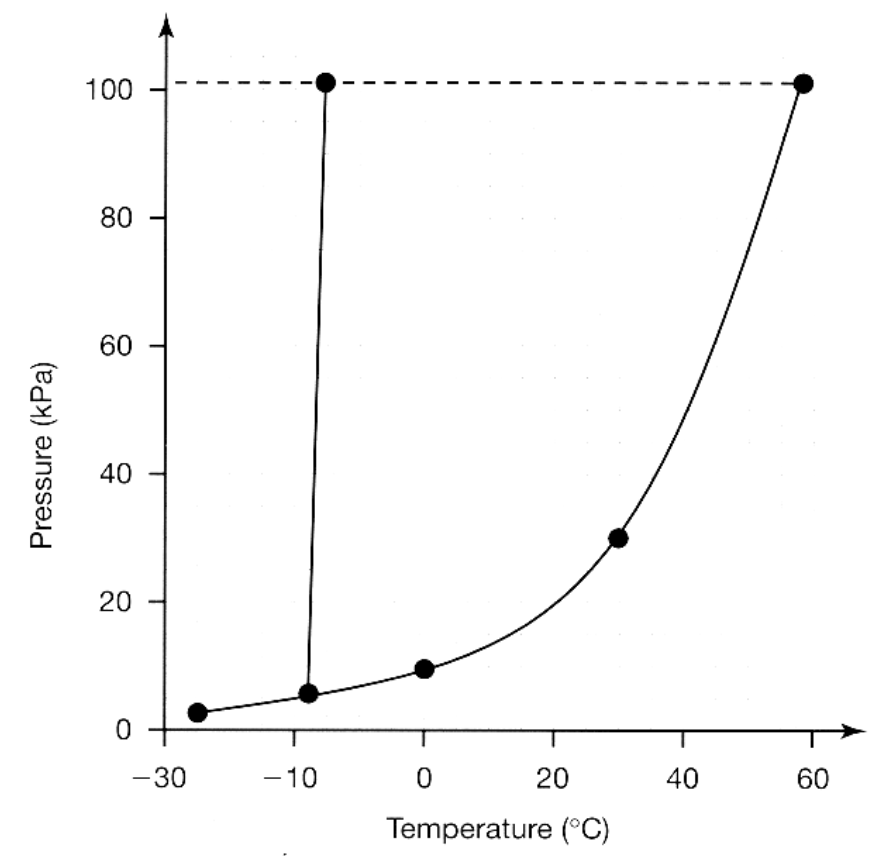
\includegraphics[scale=0.25]{br_phase}
\end{center}

a) Label each region as solid, liquid, or gas.

b) Label the triple point, melting point, and boiling point at 40 kPa.

\vspace{2in}

\textbf{Unit Concentrations}

6) A solution is prepared by missing 100.0 g of H$_2$O and 100.0g of ethanol (CH$_3$CH$_2$OH).
Determine the mole fraction of each substance.

\vspace{2in}

7) Calculate the molality of a solution containing 16.5 g of dissolved naphthalene (C$_{10}$H$_8$)
in 54.3 g benzene (C$_6$H$_6$).

\vspace{1.5in}

8) Find the molality of 18.0 M H$_2$SO$_4$. This solution has a density of 1.84 g/mL.

\vspace{1.5in}

\textbf{Valence Bond Theory}

9) Determine the hybridized orbitals of the central atom for each of the following molecules:
SO$_4^{-2}$,  PO$_3^{3-}$, NO$_2^-$, and CO$_2$

\vspace{1.5in}

10) Describe the naunce differences between the Valence Bond Theory and Molecular Orbital Theory.

\vspace{2.5in}

11) How many sigma and pi bonds are in the molecule below?

\begin{center}
  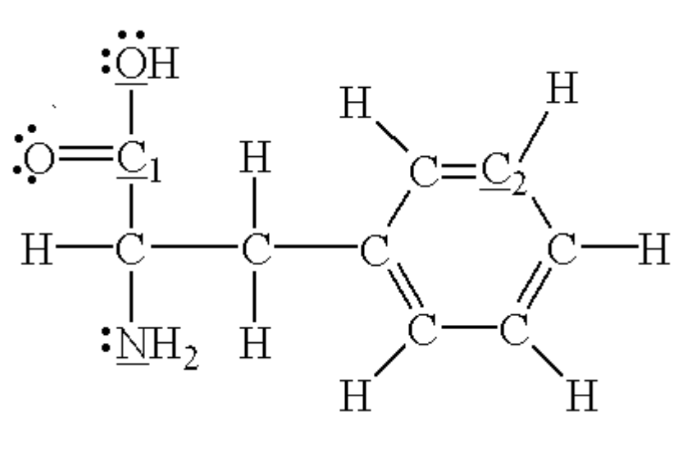
\includegraphics[scale=0.3]{sig_pi}
\end{center}

12) Use the molecular orbital diagram of Li$_2$ to sketch the Li$_2^+$ and
Li$_2^-$ ions. Compare the stability, bond strength, and magnetic properties
of each ion specie.

\begin{center}
  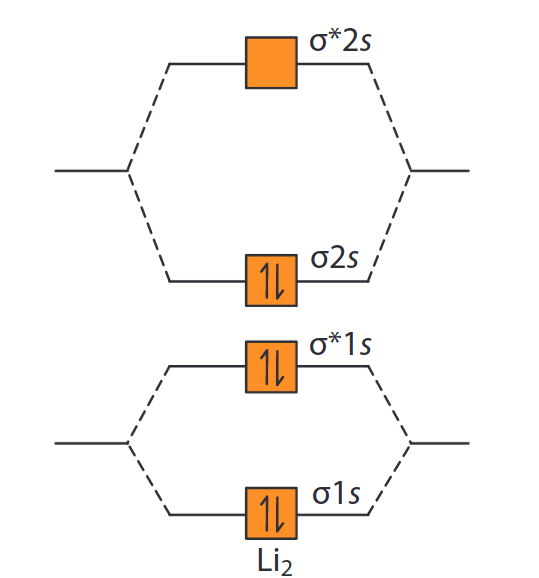
\includegraphics[scale=0.3]{li_mo}
\end{center}

\newpage

\textbf{Colligative Properties and Osmotic Pressure}

13) The freezing point of a glucose solution (C$_6$H$_{12}$O$_6$) is -10.3$^\circ$C.
The density of the solution is 1.50 g/mL. What is the molarity of the glucose solution?
K$_f$ of water is 1.86 $^\circ$C kg/mol.

\vspace{2in}

14) What is the osmotic pressure of a solution prepared by adding 13.65 g of
sucrose (C$_{12}$H$_{22}$O$_{11}$) to water to make 250. mL of solution at 25$^\circ$C.
Hint: Use $\Pi = iMRT$

\vspace{2in}

15) For the image below, there is pure water and glucose solutions separated by a
semipermeable membrane. Describe what will happen to the water level of each solution
once equilibrium is achieved.

\begin{center}
  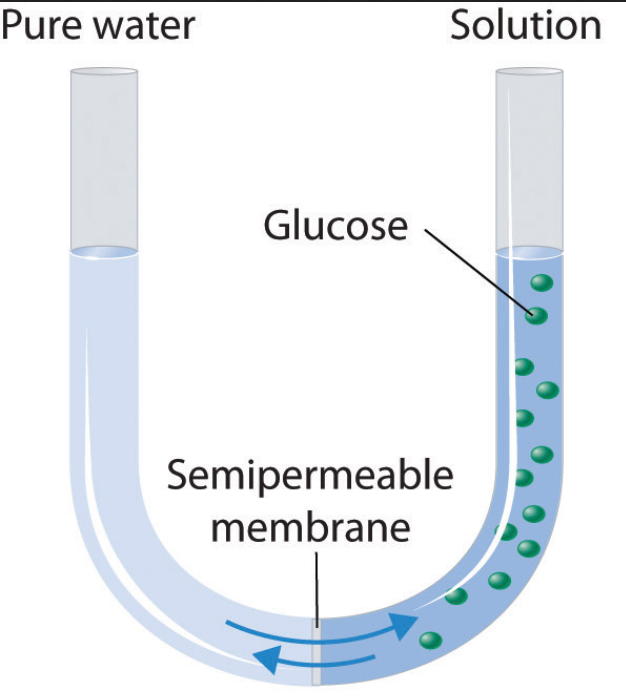
\includegraphics[scale=0.25]{osmotic_press}
\end{center}

\end{document}
